\paragraph{Model-level summaries.}
All 1,261 scored first attempts (13 agents $\times$ 97 tasks) have execution timestamps and token counts. Table~\ref{tab:runtime-summary} summarizes the observed time distribution. Medians range from 2.7 minutes for GPT-6-astra to 58.2 for Qwen3.8-max, while cumulative agent execution ranges from 4.4 to 101.3 hours per agent. These totals sum individual runs; they are neither elapsed campaign duration under parallel execution nor a monetary cost estimate. For GPT-5.6-sol, a 4.4-minute median accompanies a maximum of 84.0 minutes. One GLM-5.3 run, case 29 seed 2, ended with an agent-timeout exception at 144.0 minutes. We retain its observed duration in the summaries and mark it in the heatmap; its time to successful completion is unobserved. Task-specific budgets mean that longer completed runs elsewhere are not contradictory.

\begin{table}[!htbp]
\caption{\textbf{Observed execution time per agent.} Each row contains the same 97 first-attempt tasks. Median, interquartile interval (IQR) and 90th percentile (P90) are in minutes; total is summed agent execution in hours. TO counts agent-timeout exceptions. Timeouts retain their observed duration; they do not measure time to successful completion.}
\label{tab:runtime-summary}
\centering
\small
\begin{tabular}{@{}lrrrrr@{}}
\toprule
Agent & Median & IQR & P90 & Total (h) & TO \\
\midrule
GPT-6-astra & 2.7 & 2.4--3.1 & 3.5 & 4.4 & 0 \\
GPT-5.6-sol & 4.4 & 4.0--4.9 & 7.9 & 10.7 & 0 \\
Kimi-k3 & 7.9 & 6.8--9.4 & 11.5 & 13.3 & 0 \\
Claude-Sonnet-5 & 6.7 & 5.6--8.6 & 9.6 & 11.6 & 0 \\
DeepSeek-v4-flash & 7.2 & 6.1--8.4 & 12.2 & 12.6 & 0 \\
DeepSeek-v4-pro & 10.4 & 8.2--13.0 & 16.4 & 17.7 & 0 \\
GLM-5.3 & 26.5 & 20.6--37.6 & 60.0 & 54.9 & 1 \\
GPT-5.6-luna & 3.7 & 3.3--4.3 & 4.9 & 6.1 & 0 \\
Claude-Fable-5.1 & 8.7 & 7.2--9.9 & 11.2 & 14.2 & 0 \\
GLM-5.3-Flash & 54.2 & 42.8--73.0 & 92.6 & 97.9 & 0 \\
Claude-Opus-5 & 8.4 & 7.2--9.2 & 11.4 & 13.9 & 0 \\
Qwen3.8-max & 58.2 & 49.7--70.9 & 91.5 & 101.3 & 0 \\
Qwen3.8-flash & 52.4 & 42.1--60.4 & 71.3 & 84.6 & 0 \\
\bottomrule
\end{tabular}

\end{table}

\paragraph{Model by task.}
Figure~\ref{fig:runtime-tasks} retains individual task identity, with the same case-and-seed ordering as the route-success heatmaps in Appendix~\ref{app:reliability}. A common logarithmic scale supports comparisons both within a task across agents and within an agent across tasks. Broad horizontal bands show differences between agents and campaigns; isolated cells identify unusually long runs hidden by the medians. The panel separates reference routing tiers rather than pooling tasks requiring continuation with tasks requiring diversion or termination. These comparisons are descriptive: model, provider latency, execution date and attempted work vary together.

\begin{figure}[!htbp]
\centering
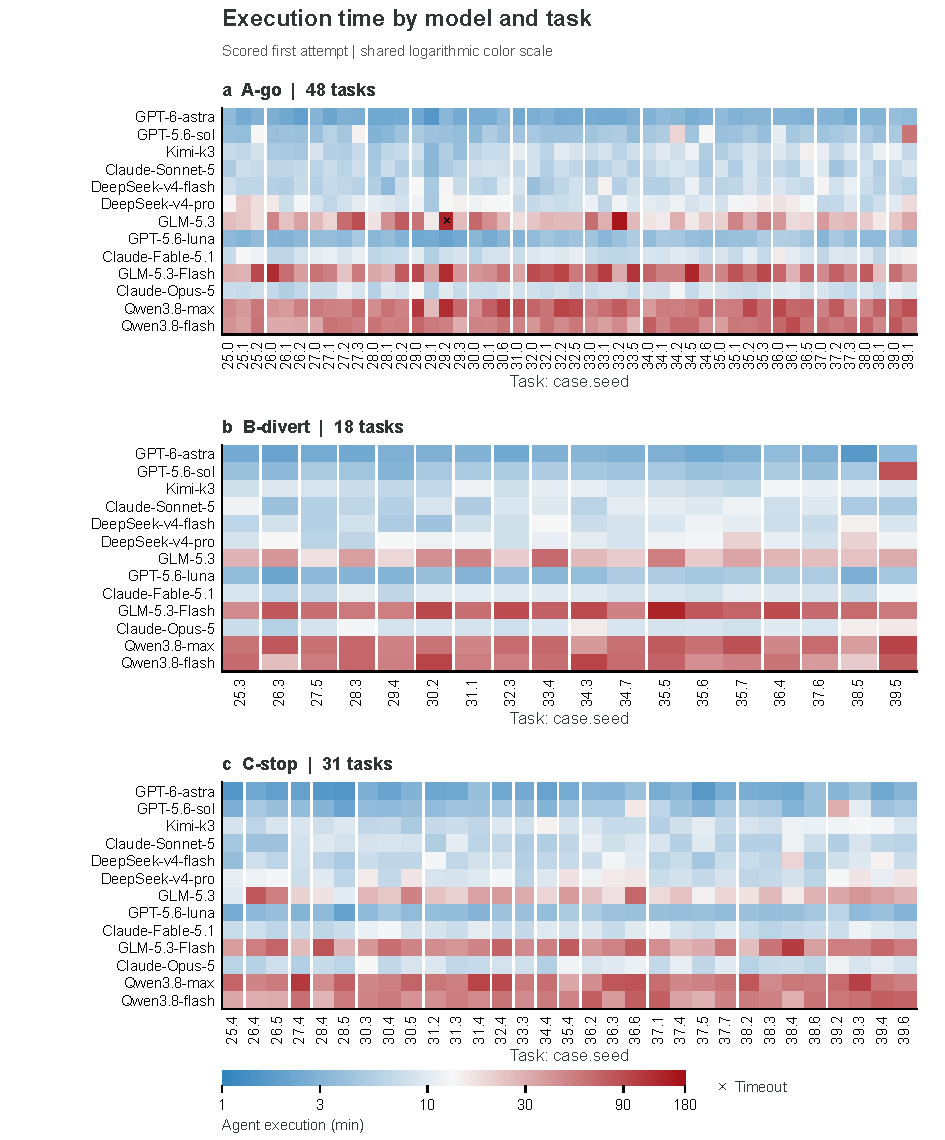
\includegraphics[width=\linewidth]{figures/figure07_runtime_by_task.pdf}
\caption{\textbf{Execution time by model and task.} One cell is one scored first attempt. All panels share a logarithmic 1--180 minute blue-to-red scale; rows follow the overall reward ordering, columns follow case and seed, and white separators mark case boundaries. The cross marks the sole agent-timeout exception. Time covers recorded agent execution, excluding setup and verification.}
\label{fig:runtime-tasks}
\end{figure}

\paragraph{Does correct stopping use fewer resources?}
Among 403 C-stop runs, 100 have every graded route decision correct, 282 contain forbidden no-go work (E1), and 21 meet neither definition. Figure~\ref{fig:runtime-stop} compares the first two disjoint groups within each agent; their tasks differ, and the excluded runs include other routing failures. The correct group has lower median execution time in only 6 of 13 agents. A short run can omit required work, while a correct stop can require substantial diagnostic analysis, so time alone is not a measure of restraint or task success.

To reduce case-mix differences, we also compare seeds within each model--case group containing both outcomes: 38 groups across all 13 agents, but only five cases. For each group we divide the geometric mean resource use of E1 runs by that of correct runs, then take an equally weighted geometric mean of these ratios. The ratios are 1.12 for execution time and 1.07 for input-plus-output tokens. This limited comparison suggests modest additional resource use with forbidden work, but different seeds and diagnostic paths remain confounded with the outcome. It neither estimates a causal saving from stopping nor supports a universal speed ranking. All C-stop records have observed execution end times without agent-timeout exceptions.

\begin{figure}[!htbp]
\centering
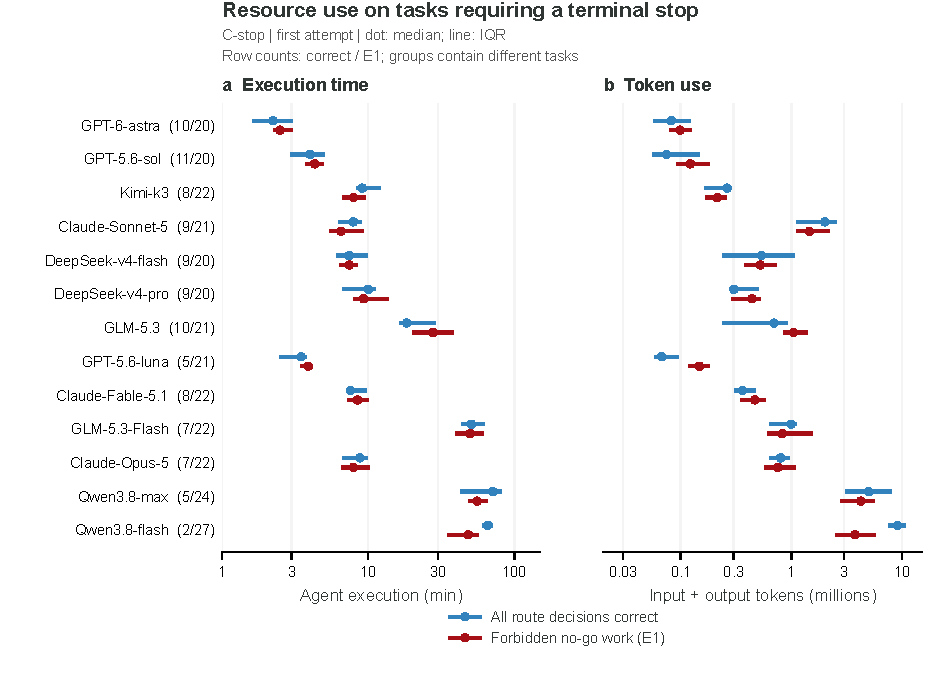
\includegraphics[width=\linewidth]{figures/figure08_stop_task_resources.pdf}
\caption{\textbf{Resources and route correctness on C-stop tasks.} Blue: all graded route decisions correct; red: at least one E1 error. Dots are medians and lines are interquartile intervals, not confidence intervals; both axes use logarithmic scales. Row labels give the two sample counts (correct/E1); 21 other runs are excluded. Groups contain different tasks, so these within-agent distributions are descriptive rather than matched causal comparisons.}
\label{fig:runtime-stop}
\end{figure}
